% Q11 -- 4x4 crossbar switch (4-bit shifter). 16 nMOS pass transistors at the
% grid crossings of 4 vertical inputs and 4 horizontal outputs; each switch has
% its OWN control => 16 control lines (the disadvantage).
\documentclass[border=10pt]{standalone}
\usepackage{tikz}
\usetikzlibrary{arrows.meta}
\begin{document}
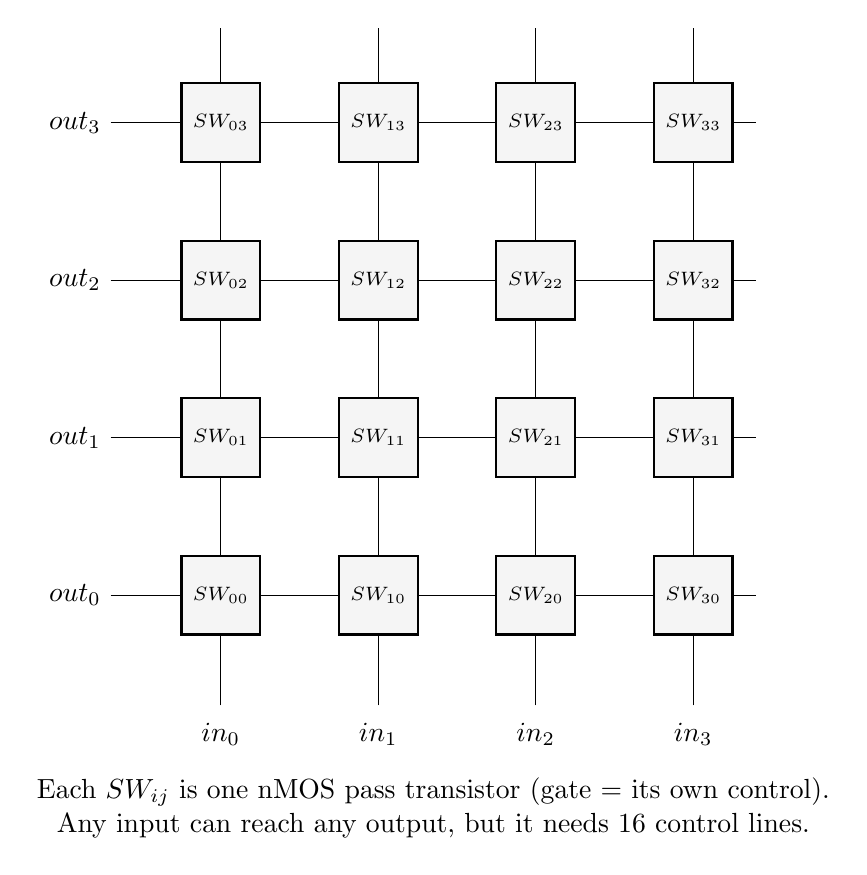
\begin{tikzpicture}[>=Latex, sw/.style={draw, thick, minimum size=1.0cm, fill=black!4}]
% vertical input lines
\foreach \j in {0,1,2,3}{
  \draw (1.6+2*\j,0.2) -- (1.6+2*\j,8.8);
  \node[below] at (1.6+2*\j,0.1) {$in_{\j}$};
}
% horizontal output lines
\foreach \i/\y in {3/7.6,2/5.6,1/3.6,0/1.6}{
  \draw (0.2,\y) -- (8.4,\y);
  \node[left] at (0.2,\y) {$out_{\i}$};
}
% switches at every crossing
\foreach \i/\y in {3/7.6,2/5.6,1/3.6,0/1.6}{
  \foreach \j in {0,1,2,3}{
    \node[sw] at (1.6+2*\j,\y) {\scriptsize $SW_{\j\i}$};
  }
}
\node[align=center] at (4.3,-1.1)
 {Each $SW_{ij}$ is one nMOS pass transistor (gate = its own control).\\
  Any input can reach any output, but it needs 16 control lines.};
\end{tikzpicture}
\end{document}
